\chapter{Result}

\section{Methods Comparison Result}

For the methods in Chapter 2, we sorted genes according to the computed measure of the strength of evidence for DE. From these sorted lists, we calculated area under ROC curve (AUC) values to evaluate the ability of these methods to distinguish genes with DE. 

To evaluate the true positive rate (TPR) and false positive rate (FPR) together, we generated receiver operator characteristic (ROC) curves based on the DE analysis results of the simulated datasets in each simulation scenario. Figure \ref{sc1_roc_01} is an example of the ROC curves we generated based on scenario 1 simulation 1 dataset. More scenario simulation ROC curves are in the Appendix. 

\begin{figure}[h!tb] 
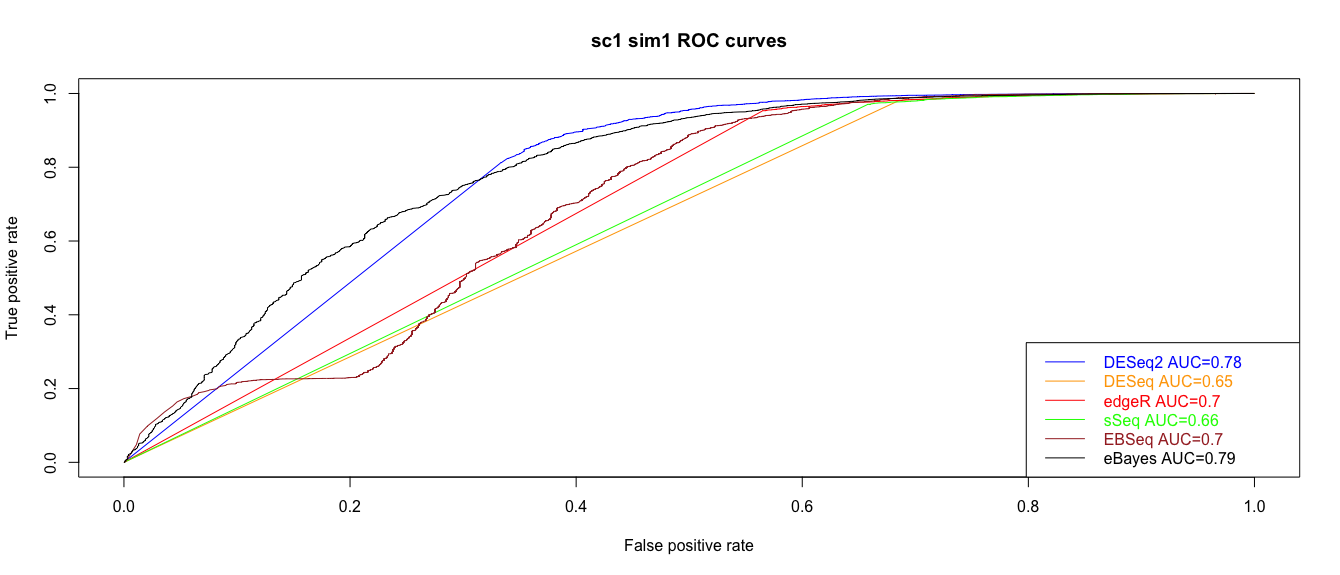
\includegraphics[height=10cm,width=15cm]{sc1_sim1_roc}
\caption{ROC curves of Simulated Datasets with $nGenes=10000, nSamples=8, pDiff=10\%$}
\label{sc1_roc_01}
\end{figure}

The most optimal ROC curve jointly displays high levels of TPR and FPR. {\tt DESeq2} and {\tt eBayes} performed equallly better than other methods when sample size is large, i.e. $nSample = 8, 16$. When we have few samples, i.e., $nSample=4$, {\tt eBayes} outperforms all other methods. 

We also evaluated the different methods with another performance metric: area under the curve (AUC) of ROC curves. Figure \ref{auc} provides the area under the ROC curve (AUC) across the 5 simulations for each of the scenario defined in \ref{tab:Scenario}. We facetted the plots by number of samples (nSample) and differential gene expression proportion (pDiff), grouped by different level of total number of genes. 

\begin{figure}[h!tb] 
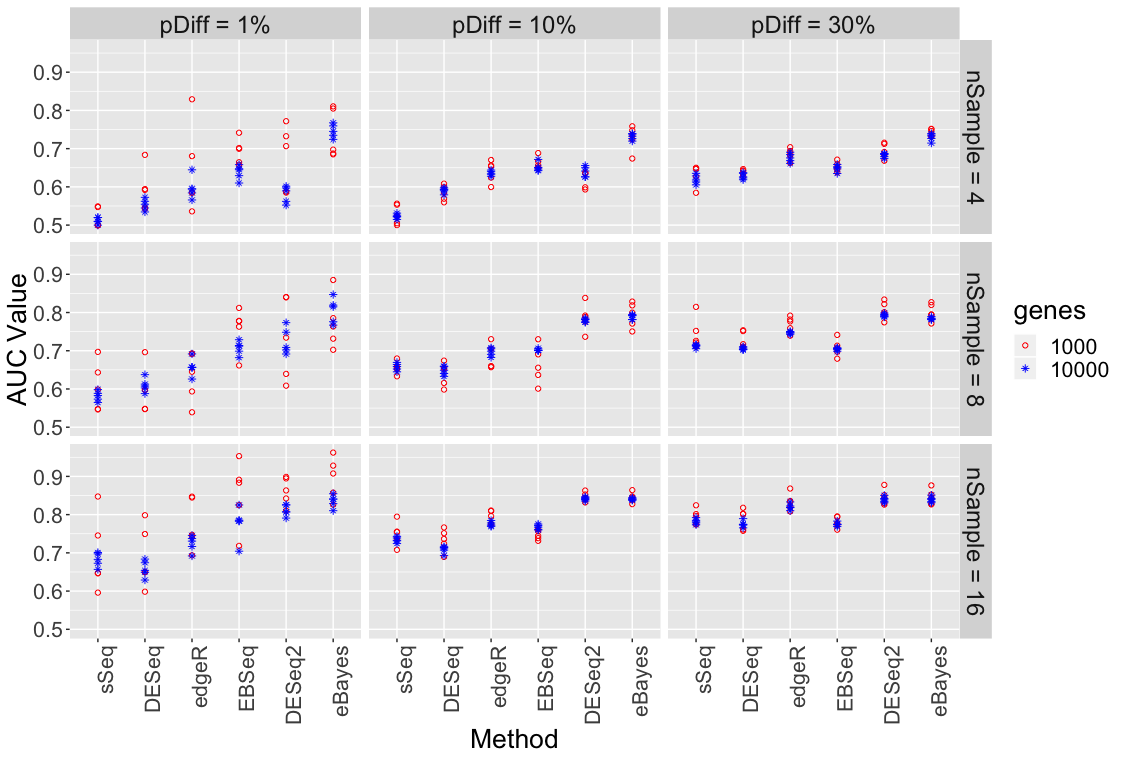
\includegraphics[height=10cm,width=18cm]{auc_plot}
\caption{AUC Plot of Simulated Datasets across Six Methods, Facetted by proportion of DE (pDiff) and number of samples (nSample), Colored by total number of Genes (nGenes)}
\label{auc}
\end{figure}

We noticed that the difference among methods shrank as proportion of DE genes $pDiff$ increases. The number of genes doesn't affect the methods performance in terms of AUC values. All methods perform better when the number of samples increases. 


\section{Discussion}

We evaluated

Try to explain the results

Limitations of this study

Future direction





\section{Appendix}

\begin{figure}[h!tb] 
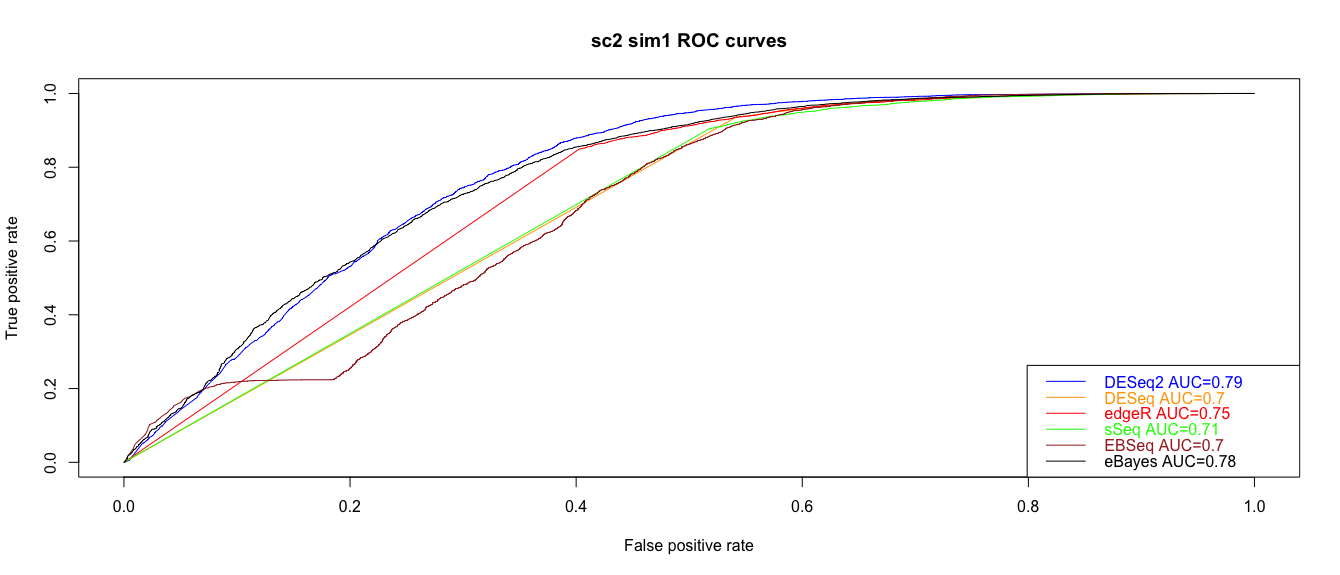
\includegraphics[height=10cm,width=15cm]{sc2_sim1_roc}
\caption{ROC curves of Simulated Datasets with $nGenes=10000, nSamples=8, pDiff=30\%$}
\label{sc2_roc}
\end{figure}

\begin{figure}[h!tb] 
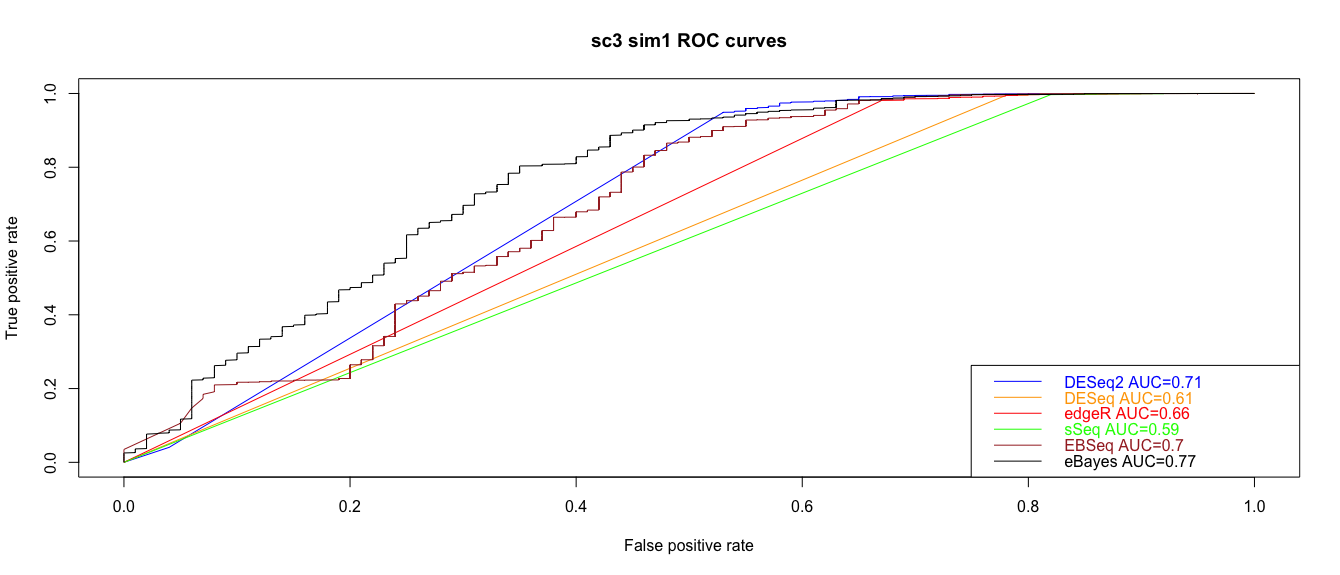
\includegraphics[height=10cm,width=15cm]{sc3_sim1_roc}
\caption{ROC curves of Simulated Datasets with $nGenes=10000, nSamples=8, pDiff=1\%$}
\label{sc3_roc}
\end{figure}


\begin{figure}[h!tb] 
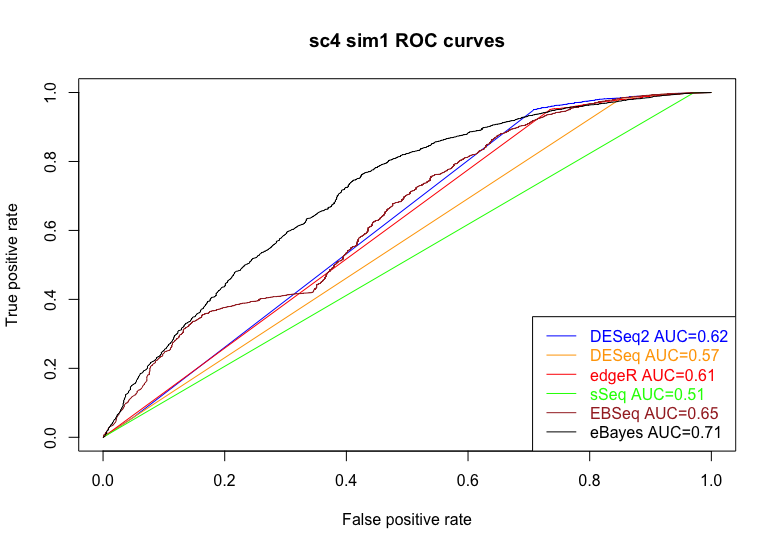
\includegraphics[height=10cm,width=15cm]{sc4_sim1_roc}
\caption{ROC curves of Simulated Datasets with $nGenes=10000, nSamples=4, pDiff=10\%$}
\label{sc4_roc}
\end{figure}


\begin{figure}[h!tb] 
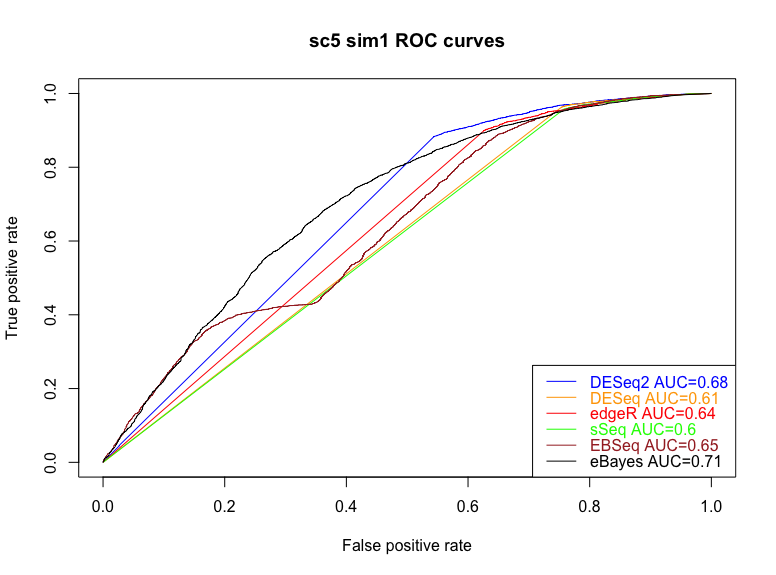
\includegraphics[height=10cm,width=15cm]{sc5_sim1_roc}
\caption{ROC curves of Simulated Datasets with $nGenes=10000, nSamples=4, pDiff=30\%$}
\label{sc5_roc}
\end{figure}


\begin{figure}[h!tb] 
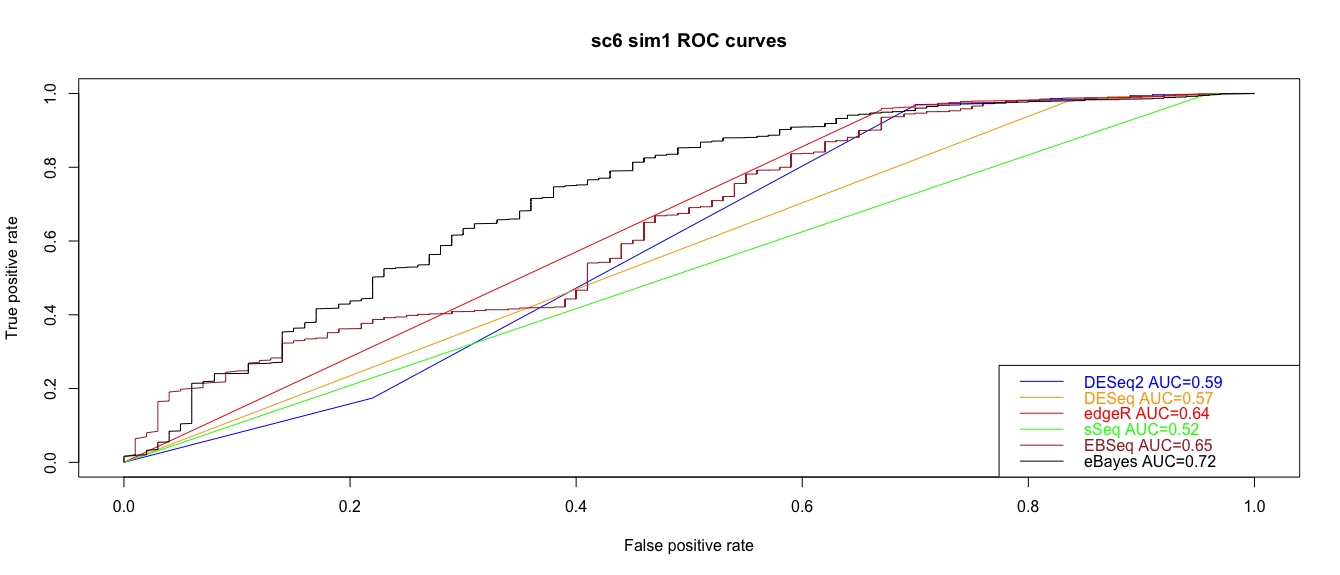
\includegraphics[height=10cm,width=15cm]{sc6_sim1_roc}
\caption{ROC curves of Simulated Datasets with $nGenes=10000, nSamples=4, pDiff=1\%$}
\label{sc6_roc}
\end{figure}

\begin{figure}[h!tb] 
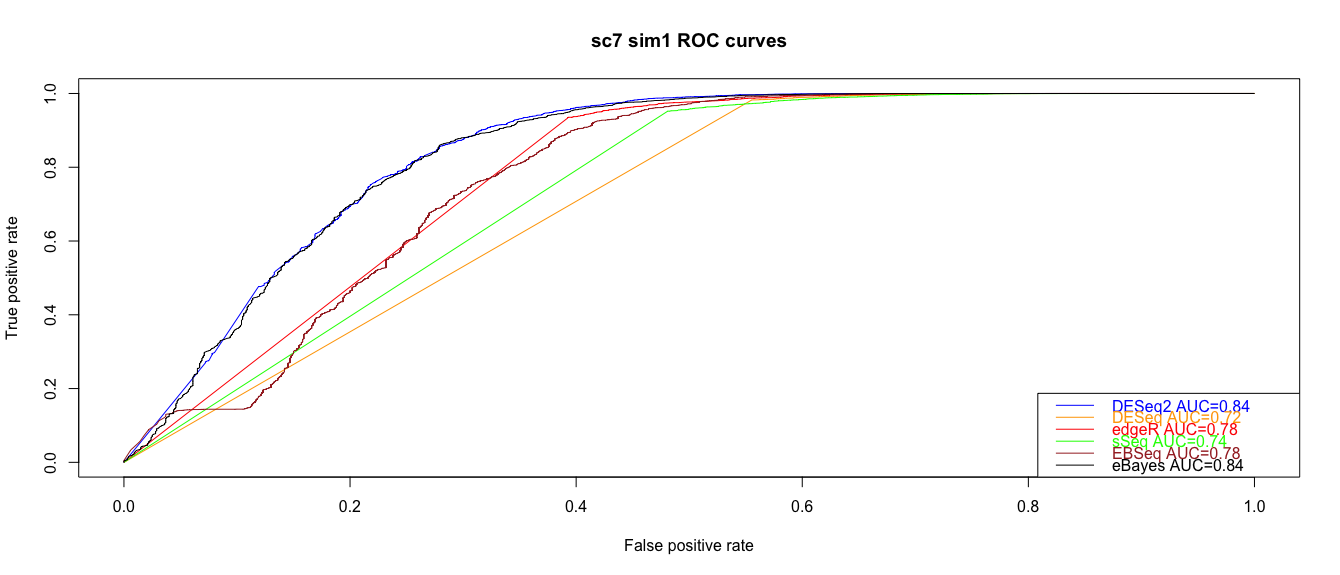
\includegraphics[height=10cm,width=15cm]{sc7_sim1_roc}
\caption{ROC curves of Simulated Datasets with $nGenes=10000, nSamples=16, pDiff=10\%$}
\label{sc7_roc}
\end{figure}

\begin{figure}[h!tb] 
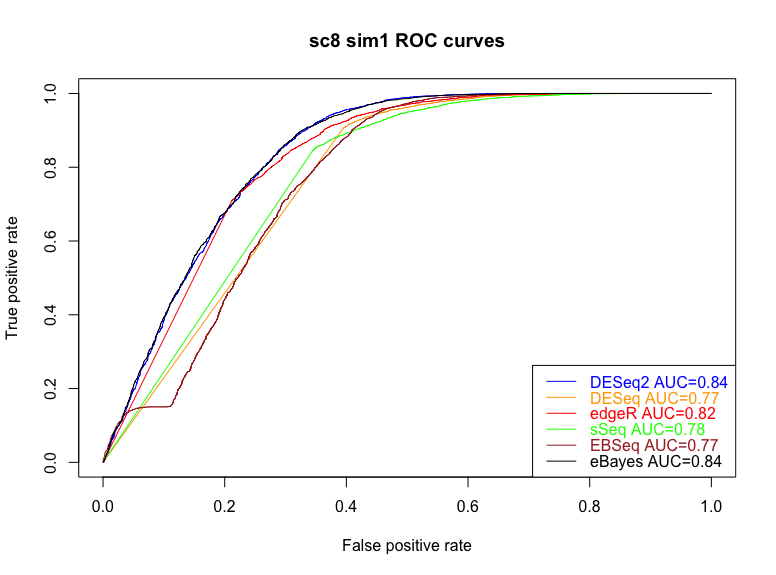
\includegraphics[height=10cm,width=15cm]{sc8_sim1_roc}
\caption{ROC curves of Simulated Datasets with $nGenes=10000, nSamples=16, pDiff=30\%$}
\label{sc8_roc}
\end{figure}

\begin{figure}[h!tb] 
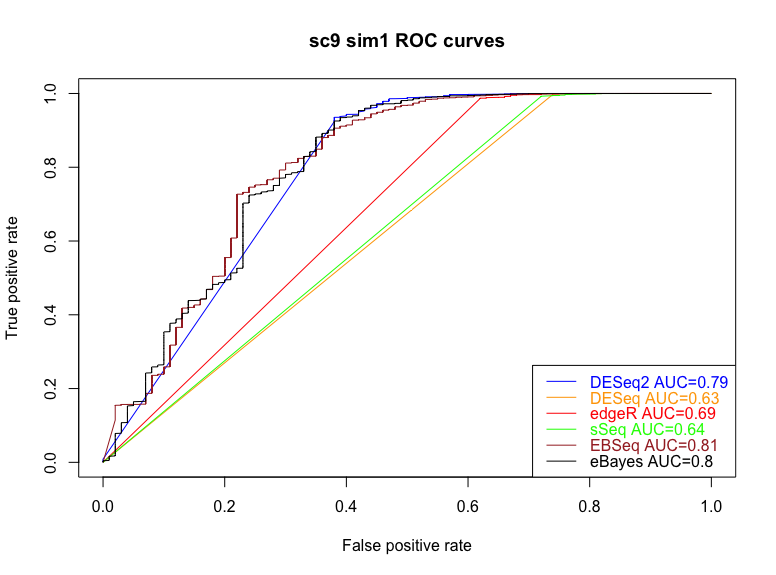
\includegraphics[height=10cm,width=15cm]{sc9_sim1_roc}
\caption{ROC curves of Simulated Datasets with $nGenes=10000, nSamples=16, pDiff=1\%$}
\label{sc9_roc}
\end{figure}


\begin{figure}[h!tb] 
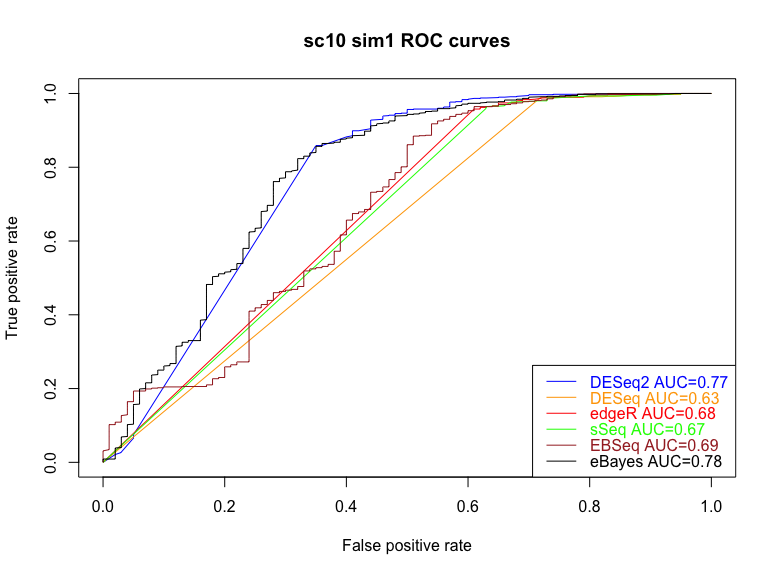
\includegraphics[height=10cm,width=15cm]{sc10_sim1_roc}
\caption{ROC curves of Simulated Datasets with $nGenes=1000, nSamples=8, pDiff=10\%$}
\label{sc10_roc_01}
\end{figure}




\begin{figure}[h!tb] 
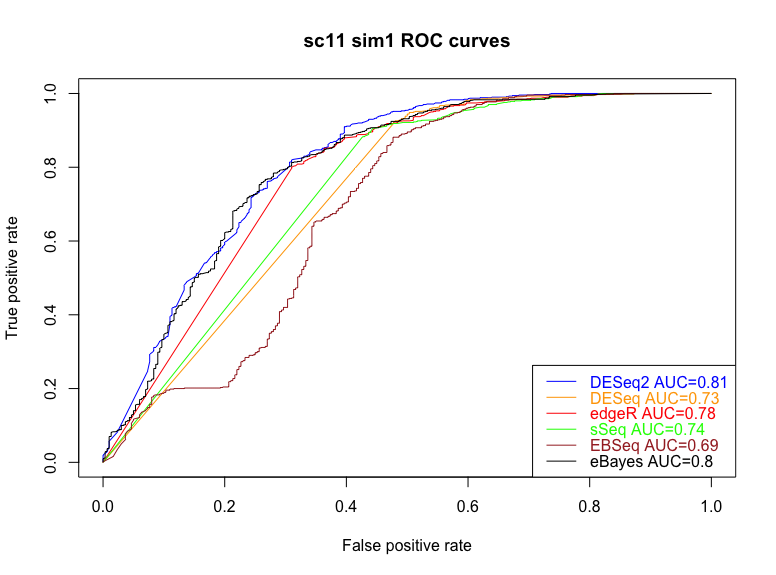
\includegraphics[height=10cm,width=15cm]{sc11_sim1_roc}
\caption{ROC curves of Simulated Datasets with $nGenes=1000, nSamples=8, pDiff=30\%$}
\label{sc11_roc}
\end{figure}

\begin{figure}[h!tb] 
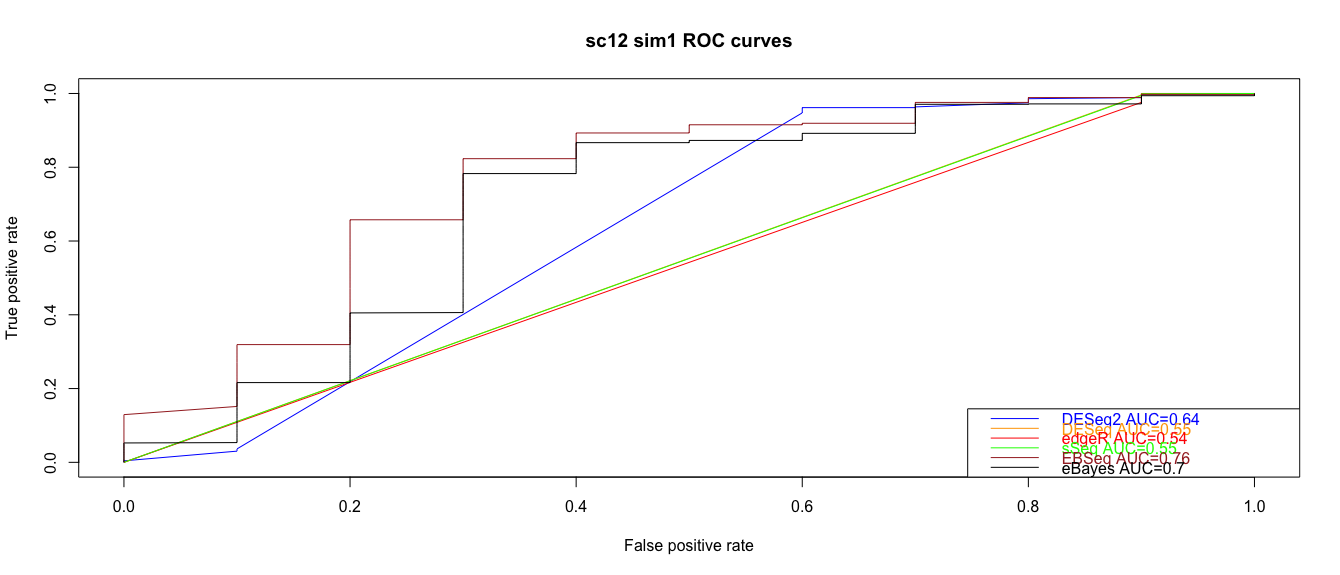
\includegraphics[height=10cm,width=15cm]{sc12_sim1_roc}
\caption{ROC curves of Simulated Datasets with $nGenes=1000, nSamples=8, pDiff=1\%$}
\label{sc12_roc}
\end{figure}


\begin{figure}[h!tb] 
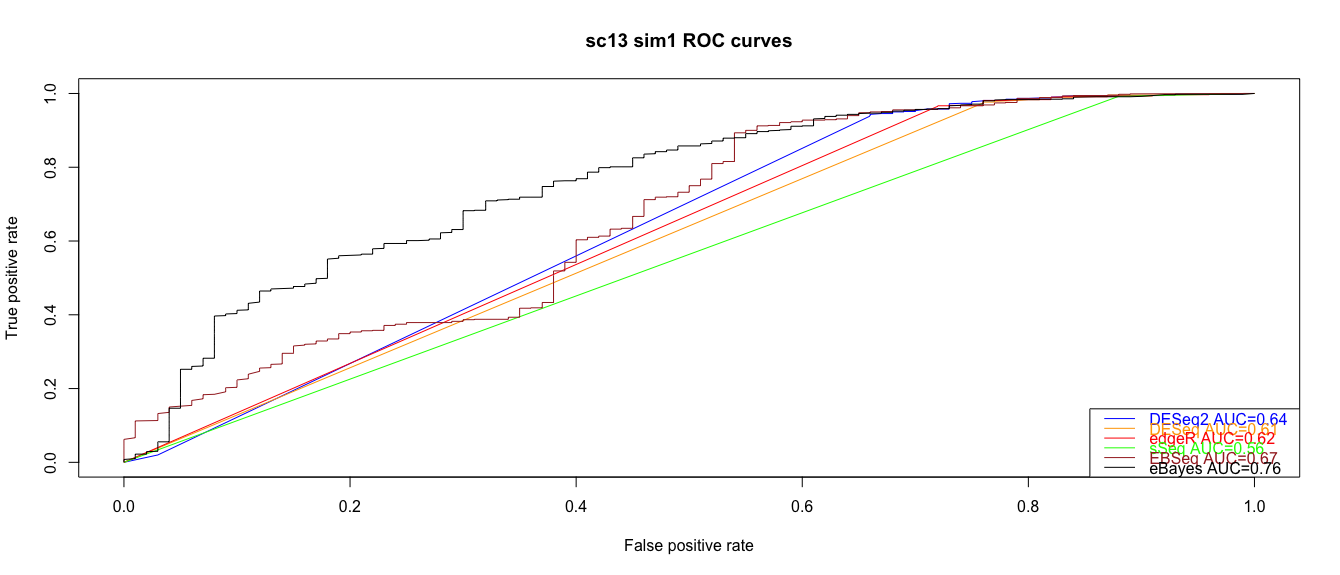
\includegraphics[height=10cm,width=15cm]{sc13_sim1_roc}
\caption{ROC curves of Simulated Datasets with $nGenes=1000, nSamples=4, pDiff=10\%$}
\label{sc13_roc}
\end{figure}


\begin{figure}[h!tb] 
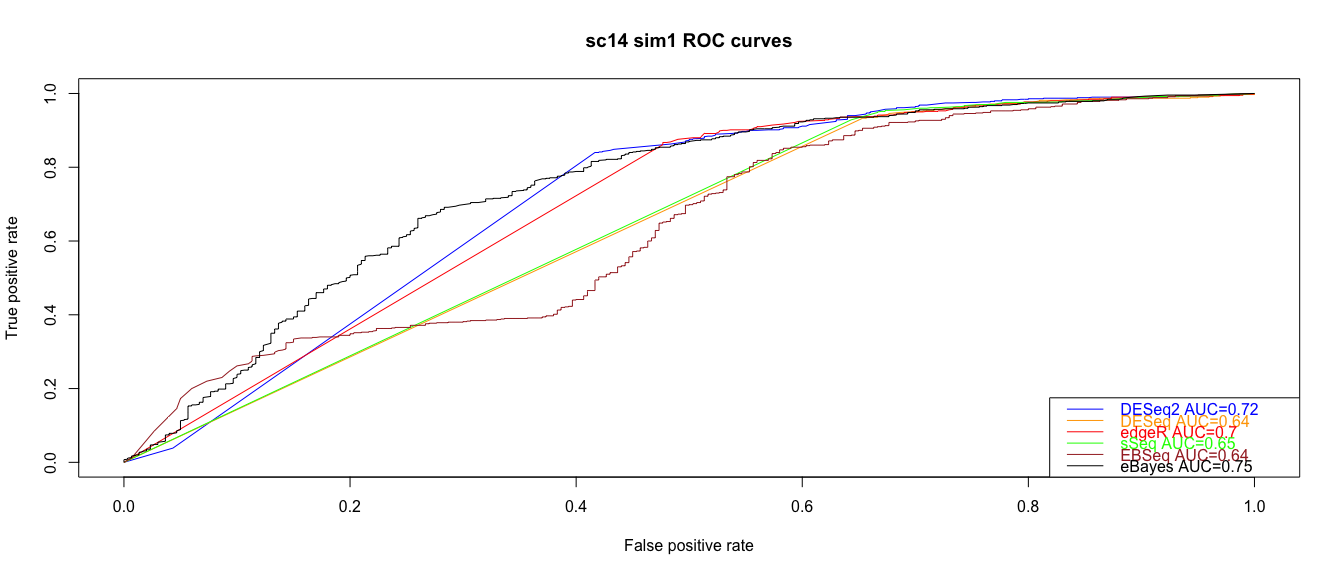
\includegraphics[height=10cm,width=15cm]{sc14_sim1_roc}
\caption{ROC curves of Simulated Datasets with $nGenes=1000, nSamples=4, pDiff=30\%$}
\label{sc14_roc}
\end{figure}


\begin{figure}[h!tb] 
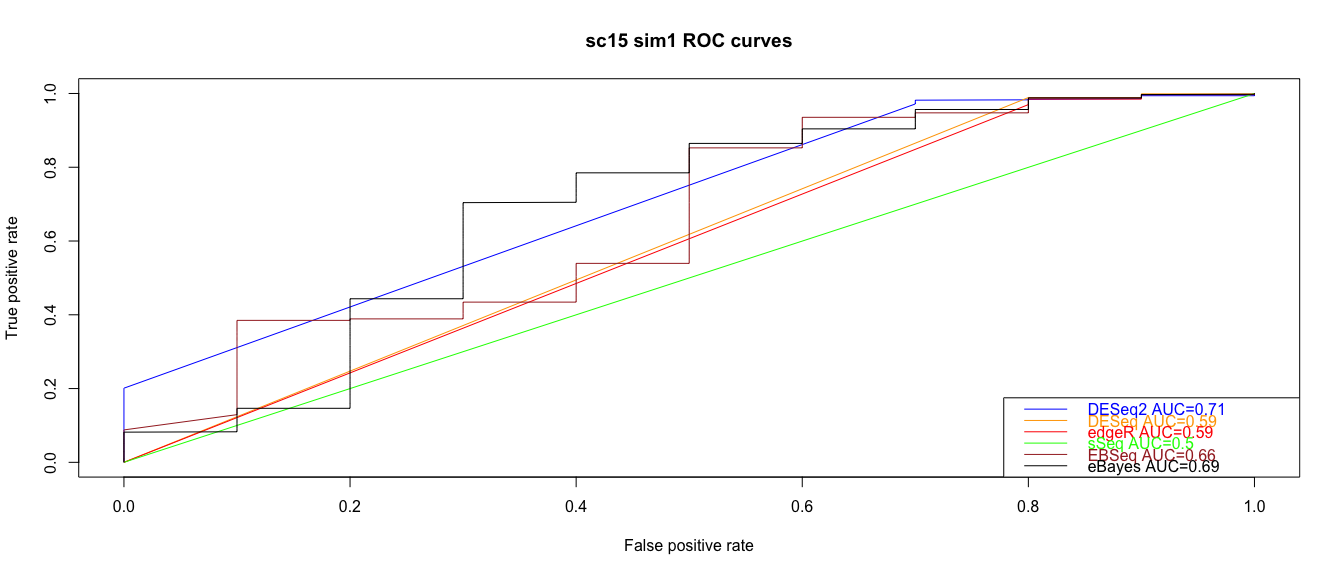
\includegraphics[height=10cm,width=15cm]{sc15_sim1_roc}
\caption{ROC curves of Simulated Datasets with $nGenes=1000, nSamples=4, pDiff=1\%$}
\label{sc15_roc}
\end{figure}

\begin{figure}[h!tb] 
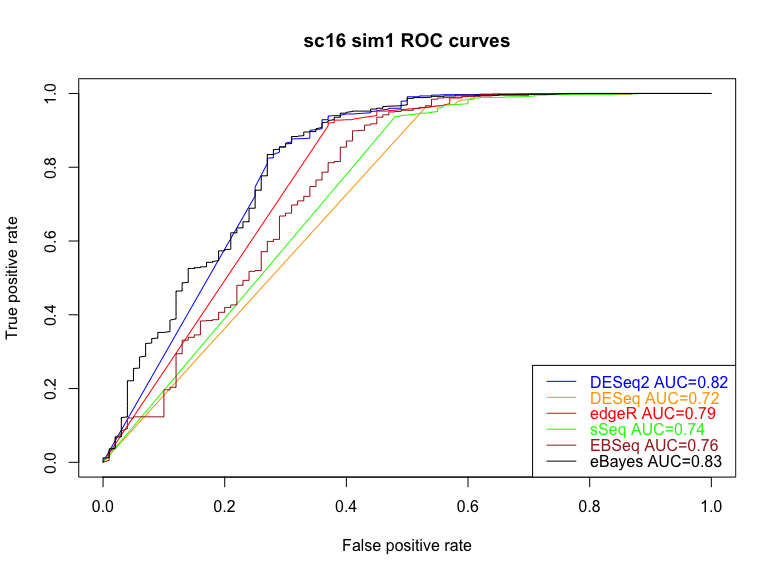
\includegraphics[height=10cm,width=15cm]{sc16_sim1_roc}
\caption{ROC curves of Simulated Datasets with $nGenes=1000, nSamples=16, pDiff=10\%$}
\label{sc16_roc}
\end{figure}

\begin{figure}[h!tb] 
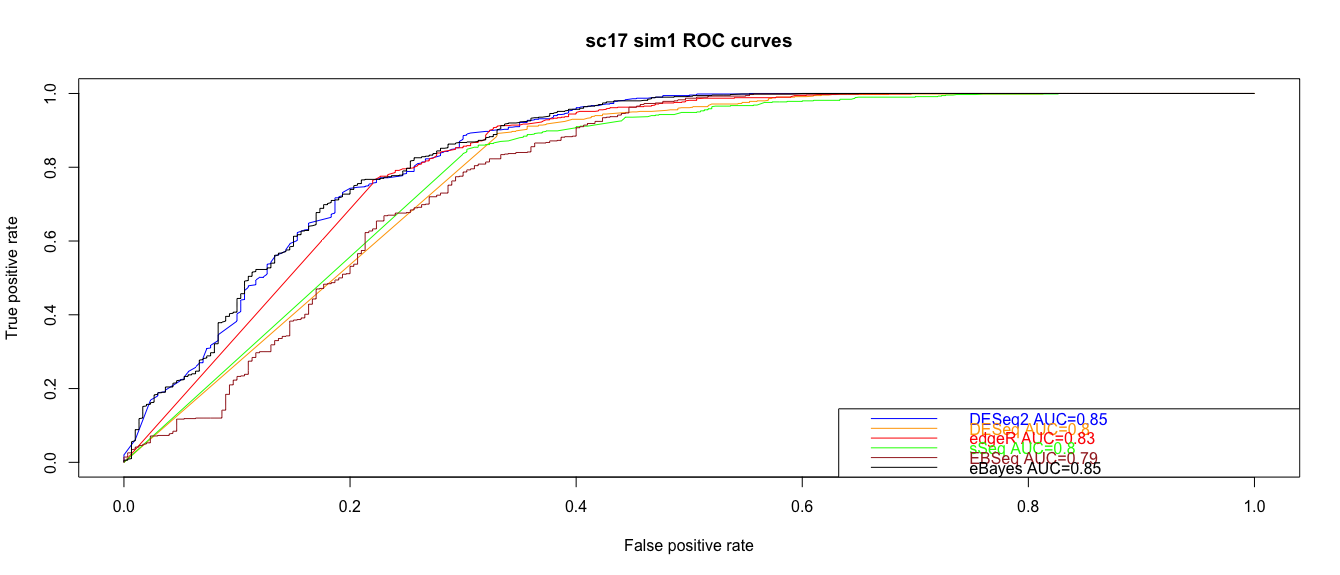
\includegraphics[height=10cm,width=15cm]{sc17_sim1_roc}
\caption{ROC curves of Simulated Datasets with $nGenes=1000, nSamples=16, pDiff=30\%$}
\label{sc17_roc}
\end{figure}

\begin{figure}[h!tb] 
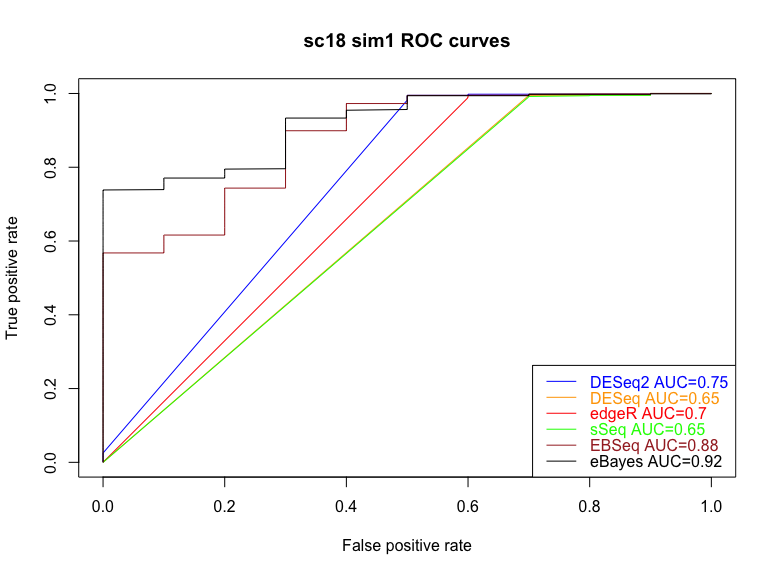
\includegraphics[height=10cm,width=15cm]{sc18_sim1_roc}
\caption{ROC curves of Simulated Datasets with $nGenes=1000, nSamples=16, pDiff=1\%$}
\label{sc18_roc}
\end{figure}
